\textbf{Question: If the rms value of the aperture jitter is 20 ps, and the input signal is a full-scale sinusoid with frequency $f_c$,
    for which values of $f_c$ will the aperture error power dominate the quantization noise power?
}
\vspace{0.5cm}

$SQNR = 20 * log_{10}(1 / (2*\pi*fc*\sigma))$

$fc = 1 / ( 10^(SQNR / 20) * 2*\pi*\sigma $

$fc$ should be greater than $1 / ( 10^(SQNR / 20) * 2*\pi*\sigma $

\vspace{1cm}
\textbf{Question: If the rms value of the aperture jitter is 20 ps, and the input signal is a 3-MHz sinusoid, for which values of the amplitude
    (in dBFS) will the aperture error power dominate the quantization noise power?
}
\vspace{0.5cm}

$\sigma_{q}^{2}=\frac{\Delta^{2}}{12}$.

$\Delta=\frac{2\cdot FS}{2^{N}}$

$\sigma_{q}^{2} = \frac{1}{12} \left( \frac{2 \cdot FS}{2^N} \right)^2 = \frac{FS^2}{3 \cdot (2^N)^2}$

$\sigma_e^2 > \sigma_q^2$

$A_{dBFS} > 66.71 - 6.02 \cdot N$


\vspace{1cm}
\textbf{Question: Simulate the effect of aperture jitter on a full-scale sinusoid with frequency $40.03905$ MHz.
    Consider two cases: $\sigma_\tau = 10$ ps and $\sigma_\tau=0.1$ ps respectively.
    Perform a 1024-FFT analysis of your data and check whether the perceived noise floor is at the expected level.
}
\vspace{0.5cm}

For $\sigma_\tau = 10ps$, the noise floor is-79.1 DBFS, and for  $\sigma_\tau = 0,1ps$ is -101 DBFS

\begin{figure}[H]
    \begin{subfigure}[t]{.5\textwidth}
        \centering
        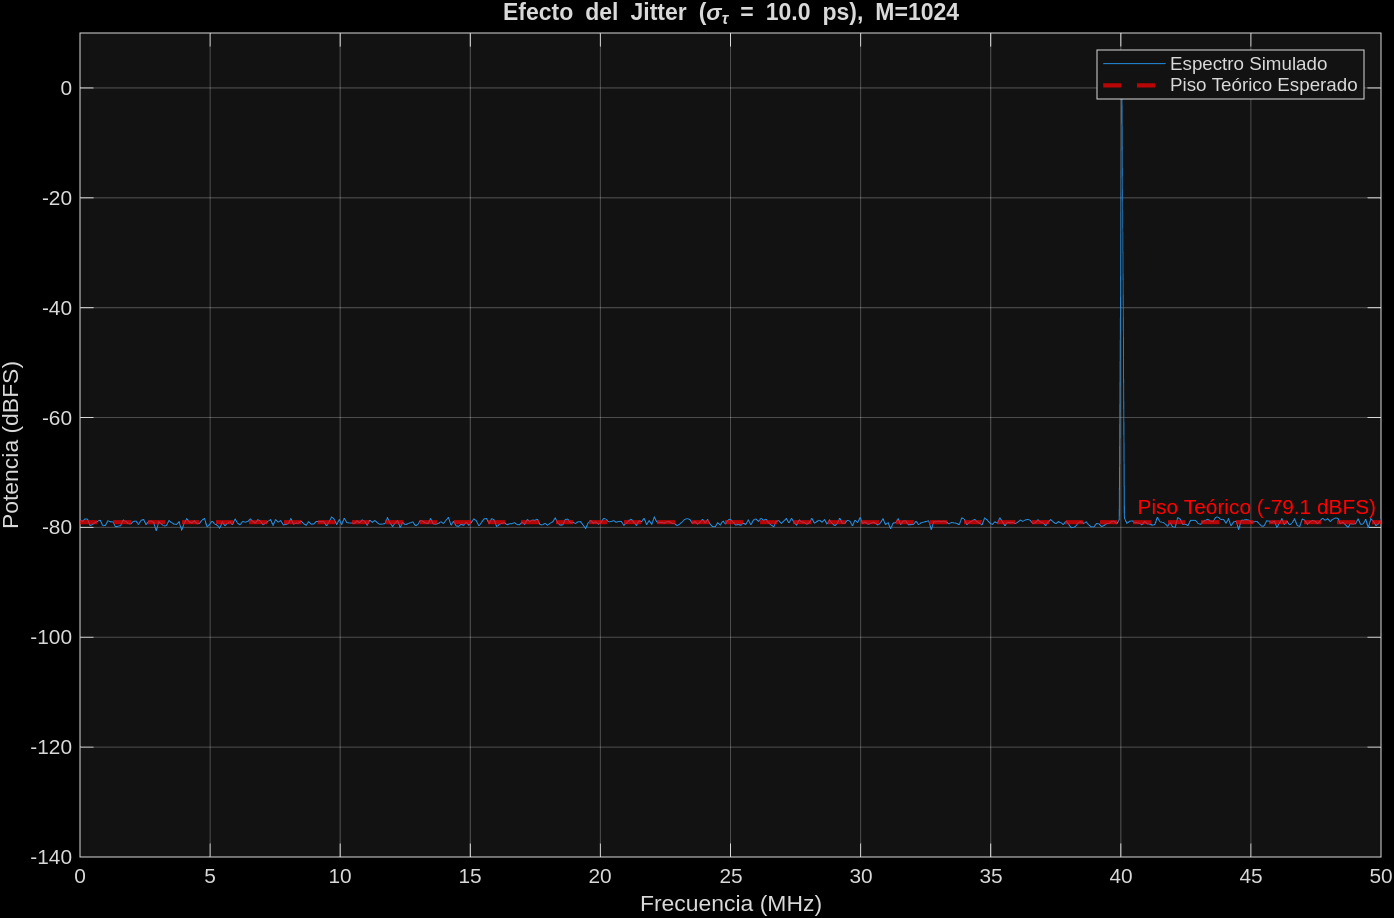
\includegraphics[width=\linewidth]{img/task6_3_10ps.png}
        \caption{$\sigma_\tau = 10ps$}
    \end{subfigure}
    \begin{subfigure}[t]{.5\textwidth}
        \centering
        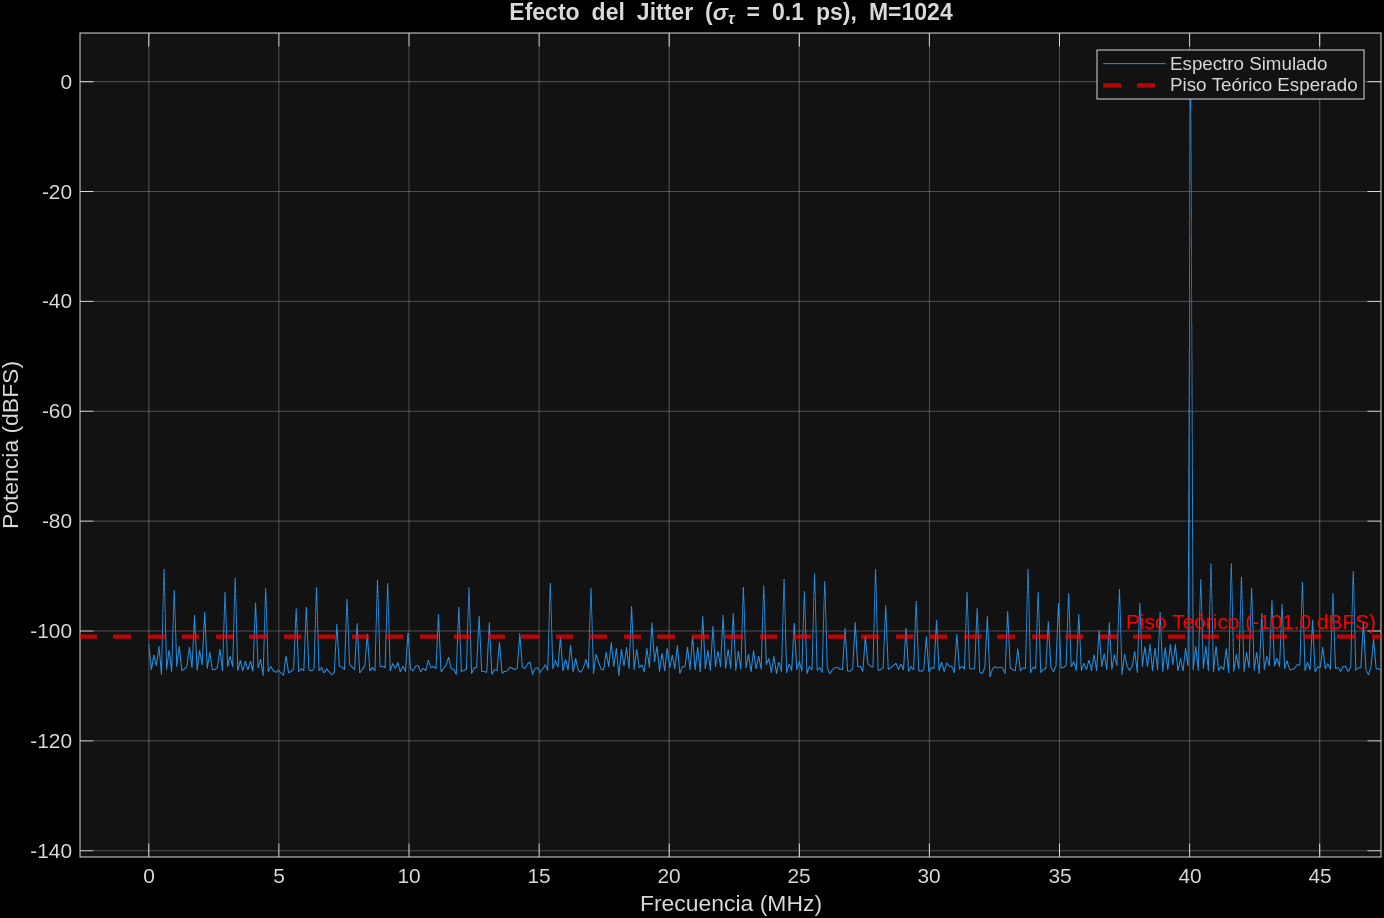
\includegraphics[width=\linewidth]{img/task6_3_01ps.png}
        \caption{$\sigma_\tau = 0,1ps$}
    \end{subfigure}

\end{figure}

\vspace{1cm}
\textbf{Question: Neglecting other possible sources of distortion, the total SNR is given by the ratio of the signal
    power to the sum of the powers of the noises due to jitter and quantization. Plot the theoretical total SNR (in dB) vs.
    input frequency over the range 0.1--100 MHz, assuming a full-scale sinusoid and for $\sigma_\tau \in \{10,20,40\}$ ps,
    $N\in \{10, 14\}$ bits (so that you should have six graphs in a single plot, whose x-axis should be in log scale).
    Comment on your results.
}
\vspace{0.5cm}

xd
